\documentclass[letter,12pt]{article}
\usepackage[letterpaper,right=1.25in,left=1.25in,top=1in,bottom=1in]{geometry}
\usepackage{setspace}

\usepackage[utf8]{inputenc}   % allows input of special characters from keyboard (input encoding)
\usepackage[T1]{fontenc}      % what fonts to use when printing characters       (output encoding)
\usepackage{amsmath}          % facilitates writing math formulas and improves the typographical quality of their output
\usepackage[hyphens]{url}     % adds line breaks to long urls
\usepackage[pdftex]{graphicx} % enhanced support for graphics
\usepackage{tikz}             % Easier syntax to draw pgf files (invokes pgf automatically)
\usetikzlibrary{arrows}

\usepackage{mathptmx}           % set font type to Times
\usepackage[scaled=.90]{helvet} % set font type to Times (Helvetica for some special characters)
\usepackage{courier}            % set font type to Times (Courier for other special characters)

\usepackage{rotating}         % sideway tables and figures that take a full page
\usepackage{caption}          % allows multipage figures and tables with same caption (\ContinuedFloat)

\usepackage{dcolumn}          % needed for apsrtable and stargazer tables from R to compile
\usepackage{arydshln}         % dashed lines in tables (hdashline, cdashline{3-4}, 
                              %see http://tex.stackexchange.com/questions/20140/can-a-table-include-a-horizontal-dashed-line)
                              % must be loaded AFTER dcolumn, 
                              %see http://tex.stackexchange.com/questions/12672/which-tabular-packages-do-which-tasks-and-which-packages-conflict

%FOR SPANISH FORMATTING (HYPHENATION ETC.)
\usepackage[spanish]{babel}
\addto\captionsspanish{\renewcommand{\figurename}{Diagrama}} % cambia Figura por Diagrama

\usepackage[longnamesfirst, sort]{natbib}\bibpunct[]{(}{)}{,}{a}{}{;} % handles biblio and references 
\AtBeginDocument{\renewcommand\harvardand{y}} % change 'author and author' by Spanish 'author y author'

\newcommand{\mc}{\multicolumn}

%% TO ADD NOTES IN TEXT, PUT % BEFORE THE ONE YOU WANT DISBALED
%\usepackage[disable]{todonotes}                            % notes not showed
\usepackage[colorinlistoftodos, textsize=small]{todonotes} % show notes
\newcommand{\emm}[1]{\todo[color=red!15, inline]{\textbf{Eric:} #1}}
\newcommand{\am}[1]{\todo[color=green!15, inline]{\textbf{Alejandro:} #1}}

\begin{document}

\title{\emph{Name recognition} en la elección de Coahuila, 2017\thanks{Una versión preliminar fue presentada el 2 de noviembre 2011 en el Center for U.S.-Mexican Studies, UCSD. Agradecemos el generoso apoyo de la Asociación Mexicana de Cultura A.C.\ así como del Sistema Nacional de Investigadores del CONACYT. Los autores somos responsables de los errores y limitaciones del estudio.}}
\author{Eric Magar  \\ ITAM \and
        Alejandro Moreno \\ ITAM 
}
\date{\today}
\maketitle

%\begin{center} \textbf{$\rightarrow$~~Preliminary draft~~$\leftarrow$} \\ (please inquire for new version, \small{\url{emagar@itam.mx}})  \end{center}

\begin{abstract}
\noindent Estudiamos el reconocimiento del nombre de candidatos al Congreso del estado de Coahuila en 2017. El fenómeno ha sido asociado con el esfuerzo del representante en su distrito para preservar su reelegibilidad. Aprovechamos la redistritación del estado que antecedió a la elección para detectar diferencias en reconocimiento atribuibles al efecto del ocupante y no al efecto de campaña. Aunque la cobertura muestral de la encuesta preeelectoral que usamos impide una separación cabal de los dos efectos, detectamos diferenciales en reconocimiento de nombre significativos y consistentes con la teoría. Ofrecemos tres diseños de investigación alternativos para que futuros estudios de opinión separen el efecto de ocupante (\emph{incumbency effect}) en elecciones que permitirán la reelección consecutiva a partir de 2018 en México. 
\end{abstract}


\onehalfspacing

\section{Introducción}

\noindent México está inaugurando la posibilidad de reelección consecutiva de sus legisladores, tanto federales como estatales, y la casi totalidad de sus alcaldes. La ciencia política norteamericana coloca a la reelección como centro neurálgico de la rendición de cuentas democrática, la clave de lo que Madison (1788)\nocite{madison.51.esp} llamó las contralorías externas del gobierno.\footnote{Vea \citet{schlesinger.1966}, \citet{mayhew.1974}, \citet{fenno.1978}, \citet{cain.etal.1987}, \citet{mccubbins.sullivan.1987}, \citet{cox.mccubbins.1993}, \citet{weingast.marshall.1988}, \citet{jacobson.1997}, entre otros.} Quienes lo ambicionan podrán permanecer un periodo adicional en el cargo si convencen al electorado de apoyarlos nuevamente. A cambio de votos el representante pone los resultados. 

Desde esta óptica, este novedoso elemento de la reforma política de 2014 tiene el potencial de inyectar muy bienvenido oxígeno a las relaciones de representación de nuestra joven democracia. Sin embargo, nada garantiza la realización del potencial. De hecho, no han faltado pesimistas que auguren su irrelevancia en México y el estrepitoso fracaso de la reforma \citep{merinoFierroZarkin2013Blog}. 

Este texto elabora las razones del optimismo y del pesimismo, y estudia Coahuila.\footnote{Hay cierto grado variación institucional entre los estados. Las instituciones pueden consultarse en \citet{magarInstReel.2017}.}

\section{La ambición política como motor democrático}

\noindent El estudio moderno del poder legislativo ha generado una parte importante de sus hipótesis a partir del prototipo de legislador de \citet{mayhew.1974}. En su obra clásica de la conexión electoral de los congresistas de EE.UU., postula al legislador como un autómata que persigue un solo objetivo: la reelección. La premisa principal del argumento es motivacional: al ocupante (una traducción con buena asonancia del ingĺés \emph{incumbent}) lo mueve exclusivamente el resorte de la ambición por permanecer otro periodo más en el Congreso. Sin poner en duda que otras preocupaciones pudieran quitarle el sueño a los ocupantes---darle sustento legal a algún programa prioritario, ascender en la jerarquía parlamentaria o pasar a la historia son algunos ejemplos obvios---Mayhew aduce que ninguna tendría remedio si el ocupante fracasara en su intento por reelegirse. No obstante su parsimonia, el modelo consigue explicar la parte medular de la conducta de los representates. 

Otra premisa del argumento es instrumental: la reelección es función de la reputación del ocupante entre sus votantes. En sistemas personalistas como el norteamericano la reputación es, sobretodo, individual---a tal grado que Mayhew descarta, de entrada, que los heterogéneos partidos norteamericanos puedan ser teóricamente interesantes \citep[aunque el revisionismo ha recuperado la relevancia de los partidos,][]{cox.mccubbins.1993,aldrich.1995}. La premisa instrumental amerita tres comentarios. 

Primero, no se trata de la totalidad de votantes del distrito que representa el ocupante, sino de un subconjunto. Importan grupos sin cuyo apoyo ganar sería mucho más difícil. \citet{cox.mccubbins.1986} los llaman \emph{core constituents} o núcleo representado. Desde esta óptica, resulta mucho más sensato y fácil trabajar en preservar la coalición que te llevó al triunfo la elección pasada que intentar construir otra nueva.

Segundo, mantener la coalición electoral exige entregar resultados, canalizando beneficios nuevos (y preservando los ya existentes) hacia el núcleo. Como en toda relación humana, el juego de percepciones importa tanto como la sustancia: el núcleo debe adscribir a su representate entre los responsables del resultado. 

Con bienes de producción colectiva, donde el esfuerzo de cada quien no es evidente de inmediato---como mucha de la política pública---la adscripción de responsabilidad está lejos de ser automática. ``La victoria tiene cien padres'' reza el proverbio. De aquí el interés que despiertan los llamados bienes particularistas, en contraposición con los más universalistas. Lo que distringue a esta clase de bienes es que su producción y/o entrega depende del esfuerzo personal del legislador \citep{haggard.mccubbins.2001}. Los ejemplos clásicos vienen de \citet{cain.etal.1987}: la gestoría distrital (\emph{service responsiveness}) y los recursos etiquetados para el distrito en el presupuesto (\emph{allocation responsiveness} o \emph{pork}). El ocupante tiene el control para canalizarlos a donde indique la lógica política, creando (esto es crucial) un vínculo claro de responsabilidad.

En la medida que la lógica de Mayhew se intersecte con problemas de adscripción, la teoría espera legisladores que dediquen una parte sustancial de su esfuerzo a cultivar su voto personal con bienes particularistas. El resultado debería ser un vínculo más cercano con su núcleo de representados que con el resto de la ciudadanía. En consecuencia, se espera también un mayor reconicimiento del diputado en el distrito que fuera de él. 

%La noción de ambición política de Mayhew es apropiada para el sistema mayoritario norteamericano, con su característico acceso competitivo y descentralizado a la boleta y carrerismo legislativo. Pero no es necesariamente apropiada para otros sistemas. Pero estos no son rasgos universales. 

%\citet{schlesinger.1966} revisó el modelo para distinguir dos clases de ambición relevantes para el estudio, la estática y la progresiva. En Mayhew hay sólo estática (permanecer en el Congreso), pero también hay políticos que aspiran a elegirse en puestos distintos. Hay evidencia de que el esfuerzo por cultivar votantes coincide con la ambición del ocupante \citep{micozzi.accountability.2013,samuels.2003}. 

%Usaremos estos elementos teóricos para guiar nuestro estudio de los candidatos a diputado local de Coahuila.

\section{La Hipótesis de Efectos Mínimos}

\begin{center}
\begin{singlespacing}
  Estamos en la posibilidad de que se apruebe la reelección\\
  y de que no se cumpla el objetivo, que es la verdadera\\
  representación y evaluación por parte de los votantes\\
  --Sen.\ Ríos Piter\footnote{Vea \url{http://www.diputados.gob.mx/sedia/biblio/prog_leg/135_DOF_10feb14.pdf}.}
\end{singlespacing}
\end{center}

\noindent No es evidente que el modelo de conexión electoral para el estudio del Congreso de EE.UU pueda extenderse a cualquier democracia, en particular a la mexicana. El escepticismo corre por dos vertientes, el candado partidista y el desinterés. Las discutimos, junto con objeciones relevantes, por separado.

\subsection{El candado partidista}

\noindent Los reformadores de 2014 otorgaron el derecho de reelección no al representante sino al partido. El ocupante mexicano podrá presentarse nuevamente ante su electorado si, y sólo si, lo postula el mismo partido que lo eligió originalmente. Este candado dota a la nomenklatura partidista de un veto absoluto sobre la renominación del representante, \emph{incluso por los demás partidos}.\footnote{Hasta que la Suprema Corte la declaró inconstitucional, la cláusula del \emph{candidato nato} en Brasil impuso la relación inversa entre el partido y el ocupante, otorgándole a éste poder para anular por completo el veto del liderazgo sobre su renominación \citep{mainwaring.1991}. Mientras que en el Reino Unido el partido nacional y el del distrito gozan de un veto mutuo sobre la nominación [*cite].}

En tal contexto, el alcalde o legislador que perciba una tensión entre los intereses de sus representados y los de su partido enfrentará un predicamento. El candado parece diseñado \emph{ex profeso} para restarle independencia al ocupante. Si optara sistemáticamente por sus representados, el ocupante se expondría a la furia del partido y, como represalia, la posibilidad de que le impidan el nuevo acceso a la boleta---la misma fuente de disciplina partidista en las cámaras que con la no reelección \citep{weldon.1997esp}. \citet{merinoFierroZarkin2013Blog} sostienen que, de hecho, el candado anulará todos los efectos benéficos de la reelección consecutiva. 

La exposición de motivos de la reforma reeleccionista omite mencionar el candado. Como a menudo ocurre con decisiones entre las cúpulas de los partidos legislativos, las intenciones de los reformadores sólo se vislumbran en boca de sus opositores. Si ninguno prosperó en removerlo, la intervención plenaria de los detractores del candado confirma la sospecha---las cúpulas temían perder el control férreo de sus ocupantes de cargos de elección popular.\footnote{El diario de los debates del 3 de diciembre 2013, sesión que discutió y aprobó el dictamen en cuestión, registra la intervención (en pro del dictamen) del Sen.\ Javier Corral (PAN--Chihuahua). Alude a legisladores oportunistas a costa de sus partidos: ``Me hubiera gustado una reelección directa,'' anunció, ``pero también creo que el dictamen se encarga de un fenómeno que no podemos negar, el transfuguismo político''. Más tarde el Sen.\ Ríos Piter (PRD--Guerrero) intentó fallidamente introducir una reserva al dictamen para eliminar el candado: ``es importante quitar[lo]'' afirmó ``[p]orque si queremos que la evaluación la hagan los ciudadanos pues no podemos dejar que dependa de un partido político'' que, en las votaciones, velará por que el ``legislador no se salga del redil.'' Vea \url{http://www.diputados.gob.mx/sedia/biblio/prog_leg/135_DOF_10feb14.pdf}.}

%Siguiendo a los apologistas de la reelección consecutiva en México desde \citet{lujambio.1996} (quizás antes), subraya un esperado efecto benéfico en la profesionalización de los legisladores.\footnote{\citet{dworak.legisladorAexamen.2003,campos.1996,careaga.1996}; \url{http://www.animalpolitico.com/blogueros-vision-legislativa/2013/12/04/reeleccion-legislativa-historia-y-estadisticas/}.} Menciona someramente el argumento de la conexión electoral, pero mantiene silencio sobre las razones del candado partidista. 

%Dip. Ricardo Monreal (oponiéndose tanto al candado como a la reelección): Si se mantiene la redacción tal y como está, lo único que se va a promover es fortalecer el cacicazgo político, fortalecer la partidocracia y generar una casta que va a ser difícil sacudirse de ella. 

Una premisa tácita detrás de la Hipótesis de Efectos Mínimos (o Nulos) es que estamos ante una maniquea dicotomía blanco (conexión electoral a la EE.UU.) o negro (impera el \emph{status quo}). Se trata más bien de una gama de grises. La plena anulación de la conexión electoral depende de que el ocupante carezca, \emph{por completo}, de recursos propios para defenderse de la cúpula. Dichos recursos, de hecho, abren la posibilidad de una negociación bilateral entre el ocupante y su partido. 

El recurso en cuestión es la competitividad electoral. \citet{zallerprizeFighters} plantea a los ocupantes como campeones del boxeo (\emph{prize fighters}): la pista electoral es un mecanismo de selección y los ganadores han demostrado mejor adaptación que sus contrincantes. Las maquinarias electorales personalistas, las dinastías políticas o el carisma son algunos de los elementos que sustentan las ``ventajas naturales'' de los ocupantes.

Desde esta perspectiva, un partido que se empecinara por coartar al campeón en su intento por reelegirse correría también el riesgo de perder el distrito. En virtud del candado, el ocupante en cuestión no podría repetir consecutivamente, pero tiene la opción de mudar su maquinaria y recursos electorales a otro partido.\footnote{Un modelo es como sigue. El voto del distrito o ayuntamiento tiene tres componentes: $p + c + o = 100$ donde $p$ es el voto esperado del partido sin la maquinaria del candidato, $c$ es el voto que moviliza el candidato con sus propios recursos y $o$ el voto esperado de la oposición. Todo candidato que controle $c \ge |p-o|$ votos estará en condición de imponerse al liderazgo del partido. La alternancia en muchos estados, distritos y municipios desde 1988 ha resultado de esta clase de desprendimientos de un partido a otro [Ver manuscrito q me dio FEE].}

Quienes cuenten con recusrsos así en suficiencia podrán negociar exitosamente con el partido sin anular la conexión electoral.La cuestión de si el tono de grises en un buen un argumento es, en todo caso, empírica. Pronto tendremos evidencia para comprobarlo. 

\subsection{El desinterés por reelegirse}

\noindent La otra vertiente es la apatía hacia la nueva institución, posibilidad que no debe descartarse. De hecho, el desinterés reeleccionista es tan común entre políticos latinoamericanos que \citet{morgenstern.2002b} y \citet{micozziPhD2009} han abogado por distinguir entre ambiciones estática y progresiva. Un vistazo a la tasa de reelección en algunos casos del continente aclara la utilidad de esta distinción de \citet{schlesinger.1966}.

\begin{table}
  \centering
%  \begin{tabular}{lccc}
%  \begin{tabular}{p{.25\textwidth} p{.18\textwidth} p{.18\textwidth} p{.18\textwidth}}
  \begin{tabular}{lccc}
%           & \mc{3}{c}{Incumbents and reelection} \\ [-.5ex]
%           & seek & succeed & return \\ \hline
                         & \mc{3}{c}{Ocupantes (\%) que} \\ 
                         & buscaron la & consiguieron    &            \\ [-.5ex]
                         & reelección  & reelegirse      & retornaron \\ [-.5ex]
    Caso                 & ($a$)       & ($b$)           & ($c=a\times b/100$) \\ \hline \\ [-1.25ex] 
    Argentina 1983--2001 & 25          &  76             &     19     \\
    Brasil 1995          & 70          &  62             &     43     \\
    Chile 1993--2000     & 71          &  83             &     59     \\
    EE.UU. 1990--2010    & 91          &  94             &     85     \\ \\ [-1.25ex] \hline
%    \mc{4}{p{.79\textwidth}}{\footnotesize{Fuentes: \citet[][:658]{jones.etal.amateurLegis.2002} para Argentina; \citet[][:415--6]{morgenstern.2002b} para Brasil y Chile; \url{https://www.opensecrets.org/overview/reelect.php} para EE.UU.}} \\ \hline
  \end{tabular}
  \caption{Querer y poder retornar al Congreso de cuatro democracias. La columna (a) reporta el porcentaje de ocupantes de la cámara baja que fueron renominados, la (b) el porcentaje de éstos que se reeligió y la (c) la tasa de retorno. Fuentes: \citet[][:658]{jones.etal.amateurLegis.2002} para Argentina; \citet[][:415--6]{morgenstern.2002b} para Brasil; \citet{naviaIncumbency.2000} para Chile; \url{https://www.opensecrets.org/overview/reelect.php} para EE.UU.}\label{T:retRate}
\end{table}

Considere, en el Cuadro \ref{T:retRate}, los valores de tres indicadores para los Congresos argentino, brasileño, chileno y estadunidense. El primer indicador es el porcentaje del total de ocupantes que volvió a contender al concluir su periodo en la cámara (columna a), que captura la ambición estática: ocupantes que intentaron repetir en el cargo. Es estática porque quienes la han tenido apostaron por desarrollar su carrera política en la cámara. Su variación es notable. Si 9 de cada 10 ocupantes estadunidenses manifiestan regularmente ambición estatica, sólo 1 de cada 4 lo hizo en Argentina desde el retorno de la democracia. Brasil y Chile ocupan posiciones intermedias, aunque más similares a EE.UU.\ que a Argentina. Como querer no es poder, el cuadro también reporta la tasa de éxito condicional (esto es, sólo entre ocupantes que buscaron la reelección, columna b). Descuella nuevamente el caso de EE.UU., donde 94 por ciento de los que lo ambicionan se reeligieron. Menos elevada, la tasa condicional de éxito de los ocupantes chilenos, de 78 por ciento, es también impresionante. En Brasil fue más moderada, de 62 por ciento. El producto los indicadores (a) y (b) produce el tercero: la tasa de retorno de ocupantes a la cámara (columna c). Los cuatro casos cubren el grueso del rango: 19 por ciento En Argentina (a pesar de una tasa condicional muy elevada) hasta 85 por ciento en EE.UU. 

Los ocupantes sin ambición estática caen en dos grupos: los de ambición progresiva (que contendieron por otro puesto) y los carentes de ambición (que se retiraron). La pregunta relevante es a cuál de estos casos se parecerá México cuando opere regularmente la reelección consecutiva. ¿Habrá escasa ambición estática, como en Argentina? Es improbable que se vuelva casi universal, como en EE.UU., ¿pero nos veremos quizás como los brasileños o los chilenos? La pregunta es empírica. En pocos años tendremos elementos para empezar a contestarla cabalmente.

\begin{table}
  \centering
  \begin{tabular}{lc}
    Año &  Retornaron (\%) \\ \hline \\ [-1.25ex]
    Constituyente &          --- \\
    1917 &           18 \\
    1918 &           25 \\
    1920 &           15 \\
    1922 &           26 \\
    1924 &           25 \\
    1926 &           30 \\
    1928 &           40 \\
    1930 &           42 \\
    1932 &           27 \\
    1934 &            0 \\ [-1.25ex] \\ \hline
  \end{tabular}
  \caption{Reelección en la Cámara de Diputados hasta 1934. Fuente: \citet{godoy.reeleccion.2014}.}\label{T:1920s}
\end{table}

La historia sugiere que hay espacio para el optimismo. El Cuadro \ref{T:1920s} reporta la tasa de retorno de diputados federales observada por \citet{godoy.reeleccion.2014} en los años previos a la prohibición de reelección consecutiva. Y la evidencia es interesante y muy sugerente. Si al principio de la serie hay similitud con la Argentina contemporánea (s\'olo 18 por ciento de constituyentes de Querétaro se integraron a la Legislatura XXVII en 1917), la tasa de retorno aceleró su crecimiento en la segunda mitad de los años 1920. Para 1928 se había más que duplicado, alcanzando 40 por ciento. Posteriormente se estabilizó y, en la antesala de la reforma no-reeleccionista, cayó.\footnote{En la elección de 1930 desaparecieron 46 por ciento de los distritos congresionales del país---de 281 integrantes, la cámara quedó con 153 solamente, vea \citet[][:23]{godoy.reeleccion.2014}. El que la tasa de retorno se mantuviera en 42 por ciento a pesar de la reducción del denominador muestra que, entre los diputados que quedaron huérfanos de distrito, hubo una proporción importante de quienes tenían ambición estática.} 

%Es indudable que la cláusula podría anular la independencia del legislador para defender los intereses de sus representados. Pero no hay tampoco garantía de ello. , Y la posibilidad de que no haya interés. En ambos casos, la pregunta es empírica. Campeones y Godoy.

%Este trabajo lleva a cabo un estudio preliminar. Aprovecha elección Coahuila 2107, primera y única hasta ahora con ocupantes en la boleta. Estudiamos una encuesta y reconocimiento de nombre. Si el diseño de la presente investigación tiene una limitación fundamental, el trabajo ofrece la ventaja de describit con detalle el diseño que permitirá superar la limitación. Bienvenido para estudiar los 24 estados que podrán tener ocupantes en la boleta en 2018. 

\section{La redistritación de Coahuila como fuente de hipótesis}

\noindent Ahora estudiaremos el reconocimiento de nombre en Coahuila, único estado que ha celebrado una elección con la reelección consecutiva vigente (sólo para legisladores). Un dato relevante para la generación de hipótesis falsificables es la redistritación. Como en el resto del país, el Instituto Nacional Electoral redibujó el mapa de los dieciséis distritos legislativos del estado en 2015 \citep{trelles.etalDatosabiertos.pyg.2016}. Así, los ocupantes que manifestaron ambición estática debieron, en consecuencia, contender en distritos más o menos diferentes de los que hasta entonces representaron, con grados variables de cambio en sus electorados.

Cuantificamos el cambio en las fronteras distritales con el índice de similitud distrital \citep[DSI por sus siglas en inglés,][]{cox.katz.2002}. Cada distrito tiene un valor propio. Se empieza por identificar, para cada distrito del mapa nuevo, aquel distrito del mapa viejo con quien más votantes comparte. Con esta pareja, obtenemos la relación de votantes que tienen en común entre la de votantes que reúnen. Así, si $\texttt{padre}_\texttt{i}$ e $\texttt{hijo}_\texttt{i}$ denotan, respectivamente, los habitantes del distrito padre y del distrito hijo, la calificación del distrito $i$ es $\text{DSI}_i = \frac{\texttt{padre}_\texttt{i} \cap \texttt{hijo}_\texttt{i}}{\texttt{padre}_\texttt{i} \cup \texttt{hijo}_\texttt{i}}$.

\begin{figure}
  \centering
    \usetikzlibrary{calc}
    \begin{tikzpicture}
      \draw (0,0)  ellipse (3 and 2);
      \node[sloped,above] at ($(0,0)+(90:3 and 2)$) {\emph{distrito$_{2014}$}};
      \draw (3,0) ellipse (3 and 2);
      \node[sloped,above] at ($(3,0)+(90:3 and 2)$) {\emph{distrito$_{2017}$}};
      \draw (-3.5,-3) rectangle (6.5,3);
      \node [text width=2cm, text centered] at (-1.25,0)   {$p=$ terreno perdido};
      \node [text width=2cm, text centered] at (4.25,0)    {$a=$ terreno adquirido};
      \node [text width=2cm, text centered] at (1.5,0)  {$c=$ terreno conservado};
      \node at (1.5,-2.5) {$h=$ huizachal};
    \end{tikzpicture}
    \caption{Cuatro terrenos claros y distintos producidos por la redistritación. En el contexto de la redistritación de Coahuila, $distrito_{2014}$ es el padre y $distrito_{2017}$ el hijo.}\label{F:venn}
\end{figure}

El Diagrama \ref{F:venn} ofrece una traducción gráfica del problema. Los óvalos representan los límites geográficos de los distritos padre ($distrito_{2014}$) e hijo ($distrito_{2017}$). Se distinguen cuatro terrenos claros y distintos. La intersección $c$ es el terreno (y su población) del padre que el distrito hijo ha conservado. A su izquierda aparece el terreno $p$ del padre que el hijo ha perdido, y la derecha el terreno $a$ que el hijo ha adquirido de otro u otros distritos del mapa viejo.\footnote{Es fácil verificar que $DSI = \frac{c}{p+a-c}$, como en \citet{cox.katz.2002}.} A falta de mejor término, llamamos al terreno $h$ que no pertence a ninguno de los óvalos el huizachal, electorado yermo para el ocupante en cuestión. El índice alcanza el valor máximo de $DSI=1$  cuando padre e hijo son idénticos (esto es, $p=a=c$) y se devaluará gradualmente conforme decrezca la intersección $c$ relativa a la unión $p \cup a$. El índice tenderá hacia el valor mínimo de cero cuando padre e hijo prácticamente no se intersecten (por construcción el cero no se alcanza porque padre e hijo dejarían de estar emparentados). 

\begin{table}
  \centering
\begin{tabular}{llrcc}
 Distrito hijo               &  Distrito padre             &       &          & Ambición  \\ [-.5ex]
 (2017)                      &  (2014)                     &  DSI  & Ocupante & revelada \\ \hline
\\ [-1.2ex]
 \textsc{xii}-Ramos Arizpe   & \textsc{v}-Ramos Arizpe     & 1.000 & Lily Gutiérrez B.      & \textbf{estática} \\
 \textsc{i}-Acuña            & \textsc{xv}-Acuña           &  .798 & Georgina Cano T.       & \textbf{estática} \\ 
 \textsc{ii}-Piedras Negras  & \textsc{xvi}-Piedras Negras &  .791 & Sonia Villarreal P.    & progresiva        \\ 
 \textsc{x}-Matamoros        & \textsc{vii}-Torreón        &  .705 & Shamir Fernández H.    & nula              \\ 
 \textsc{xiv}-Saltillo       & \textsc{i}-Saltillo         &  .700 & Javier Díaz G.         & \textbf{estática} \\ 
 \textsc{ix}-Torreón         & \textsc{viii}-Torreón       &  .650 & Irma Castaño O.        & nula              \\ 
 \textsc{vii}-Matamoros      & \textsc{vi}-Torreón         &  .618 & Verónica Martínez G.   & nula              \\ 
 \textsc{xvi}-Saltillo       & \textsc{ii}-Saltillo        &  .553 & Francisco Tobías H.    & nula              \\ 
 \textsc{iii}-Sabinas        & \textsc{xiii}-Múzquiz       &  .551 & Antonio Nerio M.       & nula              \\ 
 \textsc{xiii}-Saltillo      & \textsc{iv}-Saltillo        &  .459 & Martha Garay C.        & nula              \\ 
 \textsc{iv}-San Pedro       & \textsc{x}-San Pedro        &  .444 & Ana Isabel D.          & progresiva        \\ 
 \textsc{v}-Monclova         & \textsc{xii}-Monclova       &  .408 & Melchor Sánchez F.     & nula              \\ 
 \textsc{vi}-Frontera        & \textsc{xi}-Frontera        &  .377 & F. `Lencho' Siller     & progresiva        \\ 
 \textsc{xiii}-Saltillo      & \textsc{iii}-Saltillo       &  .236 & José María Fraustro S. & nula              \\ 
 \textsc{ix}-Torreón         & \textsc{ix}-Torreón         &  .204 & Luis Gurza J.          & nula              \\ 
 \textsc{iii}-Sabinas        & \textsc{xiv}-Sabinas        &  .197 & Martha Morales I.      & nula              \\ 
 \\ [-1.2ex] \hline
\end{tabular}
\caption{Indice de similitud distrital de Coahuila}\label{T:dsi}
\end{table}

El Cuadro \ref{T:dsi} reporta la similitud distrital de Coahuila. Operacionalizamos el índice mediante secciones electorales---la encuesta que usamos identifica la sección de registro del entrevistado.\footnote{El valor del índice arroja la proporción de secciones compartidas por padre e hijo respecto de la unión de sus secciones. Si las secciones electorales tuvieran idéntica población, nuestra operacionalización sería idéntica a la de Cox y Katz, que usan la población compartida en vez del número de secciones compartidas. Conforme crece la heterogeneidad poblacional de las secciones, también lo hace la discrepancia entre las dos versiones del $DSI$. Las secciones del país suelen tener poblaciones relativamente homogéneas: 99 por ciento de las secciones tenían en el censo 2010 una población total que oscilaba entre los 100 y los 5,700 habitantes.} Como ordena los distritos por índice ascendente, la mediana se encuentra entre el \textsc{iii} y el \textsc{xvi}) y comparte 55 por ciento de las secciones que reúne con su padre. La similitud se antoja baja: si el ocupante de este distrito aspirara a reelegirse y conociera personalmente a todos los que representó formalmente, reconocería solo a 55 por ciento de su nuevo electorado. El rango inter-cuartiles del DSI es .4--.7. 

Es interesante notar que, aunque sólo tres de dieciséis ocupantes buscaron reelegirse, todos lo hicieron en distritos con más alta similitud---como lo espera la conexión electoral. 

\begin{table}
  \centering
  \begin{tabular}{cccc}
    & Efecto &       Efecto &        Efecto \\ [-.5ex]
    & del ocupante & de la campaña & total\\ \hline
    \\ [-1.2ex]
    1 & $c>a$   & $c=a$  & $c>a$   \\
    2 & $c>p$   & $c>p$  & $c>p$   \\
    3 & $c>h$   & $c>h$  & $c>h$   \\
    4 & $p~?~a$ & $p<a$  & $p~?~a$ \\
    5 & $p>h$   & $p=h$  & $p>h$   \\
    6 & $a>h$   & $a>h$  & $a>h$   \\ \\ [-1.2ex] \hline 
  \end{tabular}
  \caption{Efectos de ocupante y de campaña sobre el reconocimiento (hipótesis). Las entradas refieren la relación esperada en el reconocimiento de nombre de un candidato en los terrenos que identifica el Diagrama \ref{F:venn}. Así, en la primera fila, el efecto de ocupante provoca un reconocimiento del candidato mayor entre los votantes del terreno conservado que entre los del terreno adquirido, diferencia que no provoca el efecto de campaña.}\label{T:hyps}
\end{table}

La redistritación permite medir efectos diferenciados en el reconocimiento del ocupante entre los votantes, que resume el Cuadro \ref{T:hyps}. Distinguimos dos fuerzas sobre el fenómeno, el efeto del ocupante, que discutimos más arriba, y el efecto de campaña. La parte fundamental del esfuerzo de la campaña legislativa se lleva a cabo en el distrito \citep{langston.nd}. Los espectaculares, la entrega de volantes, las camisetas de regalo, las pintas en bardas, los encuentros con vecinos o la compra de votos son algunos ejemplos de este esfuerzo localizado. Contribuirán a dar a conocer al candidato entre gente que lo desconocía antes de la campaña, aumento que se circuscribe al distrito (hijo) mismo. Esto genera las primeras predicciones.

Si cojes al azar un elector y vive en los terrenos $c$ o $a$ (el distrito hijo) tendrá una probabilidad sustancialmente mayor de reconocer al candidato que si viviera en $p$ o en $h$. Incluso no hay razones para esperar que el efecto de campaña per se derive en una diferencia en la probabilidad de reconocimiento entre las zonas $c$ y $a$. Los renglones 1 y 2 de la segunda columna del cuadro resumen esto como $c=a>p$. 

Pero a diferencia de la campaña, que ocurre integralmente en el nuevo distrito, el efecto del ocupante tambien se resiente, en algún grado, en el terreno $p$. Antes de conocerse la redistritación, el ocupante representó tanto a $c$ como a $p$. Al ver el nuevo mapa descubrirá que ha perdido $p$, y esto lo orilla a ajustar sus esfuerzos. No hay razón de cultivar más su voto en la zona $p$ y ahora debe hacerlo en la $a$. Sin embargo, el esfuerzo previo en $p$ (que incluye el efecto de la campaña \emph{anterior}) no se desvanece de inmediato. Y a diferencia de $c$, que experimenta dicho esfuerzo a lo largo de tres años íntegros, el terreno $a$ lo experimenta menos tiempo. Los renglones 1 y 2 de la primera columna resumen las expectativas de este efecto: $c>a$ y $c>p$. 

p ? a

> h

Los ocupantes repostulados experimentan la suma de los efectos (idéntica a las relaciones de la columna izquierda), los rivales experimentan sólo los efectos de campaña. Vea el texto.



%% \begin{table}
%%   \centering
%%   \begin{tabular}{lrrrr}
%%                & \mc{2}{c}{Contendió de nuevo}           &           &       \\ [-.5ex]
%%     Diputado   &        en un distrito & en un municipio & Se retiró & Total \\ \hline
%%     de mayoría &                     3 &            3    &        10 &    16 \\
%%     de RP      &                     0 &            3    &         6 &     9 \\ \hline
%%   \end{tabular}
%%   \caption{Ocupantes con ambición estática, progresiva o nula} \label{T:ambition}
%% \end{table}

El Cuadro \ref{T:ambition} resume la ambición revelada por los legisladores en funciones en Coahuila en 2017. De los dieciséis diputados que representaban un distrito (todos del PRI, que ganó un carro completo en 2014), tres aspiraron a reelegirse como diputados, tres a elegirse como alcaldes, y diez se retiraron. Y tres de nueve diputados de lista aspiraron a volverse alcaldes. A pesar de la posibilidad que abrió la reforma, entre los diputados que no se retiraron, los de ambición progresiva duplicaron a los de ambición estática mostraron ambición progresiva---transitaron la ruta tradicional del llamado ``chapulineo'', que antes era la única disponible.

Terminología: ocupante es un candidato que ha representado un territorio en el periodo que concluye tras la elección y que compite por la reelección; rival es todo candidato que no es ocupante.  



%\singlespacing

%% \begin{description}
%%   \item [Hipótesis 1] Manteniendo lo demás constante, el reconocimiento de un ocupante sigue los patrones siguientes:
%%     \begin{enumerate}
%%       \item es mayor entre votantes del terreno $c$ que entre los del $h$
%%       \item es mayor entre votantes del terreno $c$ que entre los del $p$
%%       \item es mayor entre votantes del terreno $c$ que entre los del $a$
%%       \item es mayor entre votantes del terreno $p$ que entre los del $h$
%%       \item es mayor entre votantes del terreno $a$ que entre los del $h$
%%       \item es mayor entre votantes del terreno $p$ que entre los del $a$
%%     \end{enumerate}
%% \end{description}

%% \onehalfspacing

%% \singlespacing

%% \begin{description}
%%   \item [Hipótesis 2] Manteniendo lo demás constante, el reconocimiento de un rival sigue los patrones siguientes:
%%     \begin{enumerate}
%%       \item es menor entre votantes del terreno $h$ que entre los demás
%%       \item no muestra diferencias significativas entre votantes de los terrenos $p$, $c$ y $a$. 
%%     \end{enumerate}
%% \end{description}

%% \onehalfspacing


\section{La encuesta y sus reactivos}

\section{Una debilidad fundamental}

Dos problemas de diseño. No contemplé medir el reconocimiento del rival de un ocupante. Tampoco incluí open seats para servir de punto de comparación. 

En principio el diferencial entre $c$ y los demás terrenos daría perspectiva para dilucidar efectos de ocupante. Pero no contaba con el modo como se diseñan las muestras de una encuesta. Todos los entrevistados de los distritos seleccionados recaen en el terreno $c$, de modo tal que los subconjuntos $p$ y $a$ están vacíos.

%% \begin{table}
%%   \centering
%%   \begin{tabular}{clllcrrrrr}
%% %      & Ocupante  & Tipo                  & Perdido & Conservado & Adquirido & Huizachal & Total \\ \hline
%%       & Ocupante        & \mc{1}{c}{Tipo (cabecera)}              & margen               & $p$ & $c$ & $a$ & $h$ & Total \\ \hline
%%     1 & Javier--PRI    & MR$\rightarrow$MR  (Saltillo)       &   \color{red}{$-12$} &  14 &  56 &  0  & 938 & 1,008 \\
%%     2 & Lily--PRI      & MR$\rightarrow$MR  (Ramos Arispe)   & \color{green}{$+14$} &   0 &  56 &  0  & 952 & 1,008 \\
%%     3 & Gina--PRI      & MR$\rightarrow$MR  (Acuña)          &   \color{red}{$-17$} &   0 &  70 &  0  & 938 & 1,008 \\ \hdashline
%%     4 & Lencho--PRI    & MR$\rightarrow$mun (Frontera)       &  \color{green}{$+8$} &  42 &  28 &  0  & 938 & 1,008 \\
%%     5 & Sonia--PRI     & MR$\rightarrow$mun (Piedras Negras) & \color{green}{$+12$} &   0 &  56 &  0  & 952 & 1,008 \\
%%     6 & AnaIsabel--PRI & MR$\rightarrow$mun (San Pedro)      &  \color{green}{$+3$} &  14 &  42 &  0  & 952 & 1,008 \\ \hdashline
%%     7 & Armando--PAN   & RP$\rightarrow$mun (Frontera)       &    \color{red}{$-8$} & 966 &  42 &  0  &   0 & 1,008 \\
%%     8 & Lariza--PAN    & RP$\rightarrow$mun (Piedras Negras) &   \color{red}{$-12$} & 966 &  42 &  0  &   0 & 1,008 \\
%%     9 & Leonel--PPC    & RP$\rightarrow$mun (Matamoros)      &    \color{red}{$-7$} & 966 &  42 &  0  &   0 & 1,008 \\ \hline
%%   \end{tabular}
%%   \caption{Los ocupantes y su terreno. El tipo distingue ocupantes de mayoría (dist) o representación proporcional y si contendieron nuevamente para la legislatura (dist) o una alcaldía (mun). El margen es la diferencia porcentual que separa segundo lugar del ganador, positivo si el ocupante ganó, negativo si perdió. Las columnas $p$, $c$, $a$, $h$ reportan el número de secciones electorales en cada una de las categorías de terreno.}\label{T:terrenos}
%% \end{table}

\begin{table}
  \centering
  \begin{tabular}{llcrrrr|rrrr}
                & Cabecera/   &                      &  \mc{4}{c}{Secciones}& \mc{4}{c}{Encuestados}  \\ 
    Ocupante    & municipio   & Margen               &  $p$ & $c$ & $a$& $h$  & $p$ & $c$ & $a$ & $h$  \\ \hline
    \hline \\[-1.8ex] 
    \mc{7}{l|}{~~A. \emph{Ambición estática (MR$\rightarrow$MR)}} \\ \hdashline
  Javier PRI    & Saltillo    &   \color{red}{$-12$} &   14 &  64 & 13 & 1,619 &  14 &  56 &  0  & 938  \\
  Lily PRI      & R. Arispe   & \color{green}{$+14$} &    0 & 117 &  0 & 1,593 &   0 &  56 &  0  & 952  \\
  Gina PRI      & Acuña       &   \color{red}{$-17$} &    0 &  78 & 21 & 1,611 &   0 &  70 &  0  & 938  \\
  \\[-1.8ex] 
    \mc{7}{l|}{~~B. \emph{Ambición progresiva (MR$\rightarrow$municipio)}} \\ \hdashline
  Lencho PRI    & Frontera    &  \color{green}{$+8$} &   83 &  41 &  0 & 1,586 &  42 &  28 &  0  & 938  \\
  Sonia PRI     & P. Negras   & \color{green}{$+12$} &    0 &  88 &  0 & 1,622 &   0 &  56 &  0  & 952  \\
  AnaIsabel PRI & San Pedro   &  \color{green}{$+3$} &   48 &  75 &  0 & 1,587 &  14 &  42 &  0  & 952  \\ 
  \\[-1.8ex]
  \mc{7}{l|}{~~C. \emph{Ambición progresiva (RP$\rightarrow$municipio)}} \\ \hdashline
  Armando PAN   & Frontera    &    \color{red}{$-8$} & 1,635 &  75 &  0 &    0 & 966 &  42 &  0  &   0  \\
  Lariza PAN    & P. Negras   &   \color{red}{$-12$} & 1,635 &  75 &  0 &    0 & 966 &  42 &  0  &   0  \\
  Leonel PPC    & Matamoros   &    \color{red}{$-7$} & 1,648 &  62 &  0 &    0 & 966 &  42 &  0  &   0  \\
  \\[-1.8ex] \hline \hline
  \end{tabular}
  \caption{Los ocupantes y su terreno. Se distingue aquéllos con ambición estática---de un distrito de mayoría (MR) a otro---y dos tipos con ambición progresiva---hacia una presidencia municipal desde una diputación de mayoría o desde una de representación proporcional (RP). El margen es la diferencia porcentual que separa segundo lugar del ganador en la elección subsecuente, positivo si el ocupante ganó, negativo si perdió. El primer conjunto de columnas $p$, $c$, $a$, $h$ reporta el número de secciones electorales (de un total de 1,710 en el estado) en cada una de las categorías de terreno. El segundo reporta el número de entrevistados en la encuesta (de un total de 1,008) en cada categoría de terreno.}\label{T:terrenos}
\end{table}


Conjugados, los dos errores de diseño impedirán distringuir entre efectos de campaña y efectos de \emph{incumbency}. 



\section{Las regresiones}

% Table created by stargazer v.5.2 by Marek Hlavac, Harvard University. E-mail: hlavac at fas.harvard.edu
% Date and time: Wed, Feb 14, 2018 - 08:56:20 PM
% Requires LaTeX packages: dcolumn 
\begin{sidewaystable}[!htbp] \centering 
\begin{tabular}{l|rrr|rrr|rrr} 
% \begin{tabular}{@{\extracolsep{5pt}}lD{.}{.}{-3} D{.}{.}{-3} D{.}{.}{-3} D{.}{.}{-3} D{.}{.}{-3} D{.}{.}{-3} D{.}{.}{-3} D{.}{.}{-3} D{.}{.}{-3} } 
%\\[-1.8ex]\hline 
%\hline \\[-1.8ex] 
\\[-1.8ex] & \multicolumn{1}{c}{(1)} & \multicolumn{1}{c}{(2)} & \multicolumn{1}{c}{(3)} & \multicolumn{1}{c}{(4)} & \multicolumn{1}{c}{(5)} & \multicolumn{1}{c}{(6)} & \multicolumn{1}{c}{(7)} & \multicolumn{1}{c}{(8)} & \multicolumn{1}{c}{(9)}\\ 
  & \multicolumn{1}{c}{Javier} & \multicolumn{1}{c}{Lily} & \multicolumn{1}{c}{Gina} & \multicolumn{1}{c}{Lencho} & \multicolumn{1}{c}{Sonia} & \multicolumn{1}{c}{A.Isabel} & \multicolumn{1}{c}{Armando} & \multicolumn{1}{c}{Lariza} & \multicolumn{1}{c}{Leonel}\\ 
\hline \\[-1.8ex] 
 conservado & 1.85^{***} & 2.37^{***} & 4.91^{***} & 3.10^{***} & 3.02^{***} & 4.59^{***} & 1.10^{*} & -.22 & 2.93^{***} \\ 
  & (.33) & (.33) & (.41) & (.43) & (.32) & (.44) & (.58) & (.75) & (.38) \\ 
  & & & & & & & & & \\ 
 perdido & 1.29^{*} &  &  & 1.27^{***} &  & 1.46^{*} &  &  &  \\ 
  & (.68) &  &  & (.47) &  & (.81) &  &  &  \\ 
  & & & & & & & & & \\ 
 ha.hecho & .86^{***} & .76^{***} & 1.46^{***} & .51^{*} & .93^{***} & .26 & .51 & .85^{***} & .26 \\ 
  & (.25) & (.27) & (.34) & (.30) & (.27) & (.34) & (.37) & (.27) & (.33) \\ 
  & & & & & & & & & \\ 
 interesa.polít & .35 & 1.03^{***} & 1.34^{***} & .82^{***} & .52^{**} & .74^{**} & .71^{**} & .28 & .57^{*} \\ 
  & (.24) & (.27) & (.34) & (.28) & (.26) & (.33) & (.36) & (.27) & (.31) \\ 
  & & & & & & & & & \\ 
 smartphone & -.27 & .37 & -.18 & -.47^{*} & .21 & -.05 & -.43 & .26 & -.42 \\ 
  & (.24) & (.27) & (.31) & (.28) & (.26) & (.31) & (.35) & (.27) & (.30) \\ 
  & & & & & & & & & \\ 
 panista & .15 & -.11 & -.03 & 1.18^{***} & .02 & .80^{*} & .78^{*} & .34 & 1.15^{***} \\ 
  & (.39) & (.41) & (.52) & (.35) & (.41) & (.44) & (.47) & (.39) & (.41) \\ 
  & & & & & & & & & \\ 
 priista & .37 & .15 & -.01 & -.21 & .17 & .74^{**} & .43 & .19 & .16 \\ 
  & (.28) & (.30) & (.38) & (.37) & (.29) & (.35) & (.41) & (.31) & (.39) \\ 
  & & & & & & & & & \\ 
 morenista & -.07 & .59 & .26 & .76 & -1.17 &  & -.26 & -1.01 & .88 \\ 
  & (.63) & (.51) & (.74) & (.55) & (1.04) &  & (1.05) & (1.03) & (.56) \\ 
  & & & & & & & & & \\ 
 constante & -3.03^{***} & -3.82^{***} & -4.45^{***} & -3.48^{***} & -3.49^{***} & -3.99^{***} & -3.87^{***} & -3.29^{***} & -3.58^{***} \\ 
  & (.25) & (.30) & (.39) & (.30) & (.28) & (.35) & (.37) & (.28) & (.30) \\ 
  & & & & & & & & & \\ 
\hline \\[-1.8ex] 
Observations & \multicolumn{1}{c}{1,008} & \multicolumn{1}{c}{1,008} & \multicolumn{1}{c}{1,008} & \multicolumn{1}{c}{1,008} & \multicolumn{1}{c}{1,008} & \multicolumn{1}{c}{1,008} & \multicolumn{1}{c}{1,008} & \multicolumn{1}{c}{1,008} & \multicolumn{1}{c}{1,008} \\ 
Log Likelihood & \multicolumn{1}{c}{-262.32} & \multicolumn{1}{c}{-231.34} & \multicolumn{1}{c}{-169.84} & \multicolumn{1}{c}{-205.60} & \multicolumn{1}{c}{-235.20} & \multicolumn{1}{c}{-175.64} & \multicolumn{1}{c}{-147.10} & \multicolumn{1}{c}{-229.85} & \multicolumn{1}{c}{-182.89} \\ 
\hline 
\hline \\[-1.8ex] 
    \multicolumn{10}{r}{\footnotesize{$^{*}$p$<$.1; $^{**}$p$<$.05; $^{***}$p$<$.01}} \\ %[-1.8ex]
\end{tabular} 
  \caption{Resultados logit} 
  \label{T:regs} 
\end{sidewaystable} 


\section{Lo que sigue}

\begin{sidewaysfigure}
  \centering
  \begin{tabular}{ccc}
    Ambición estática & Ambición progresiva MR & Ambición progresiva RP \\ \hline
    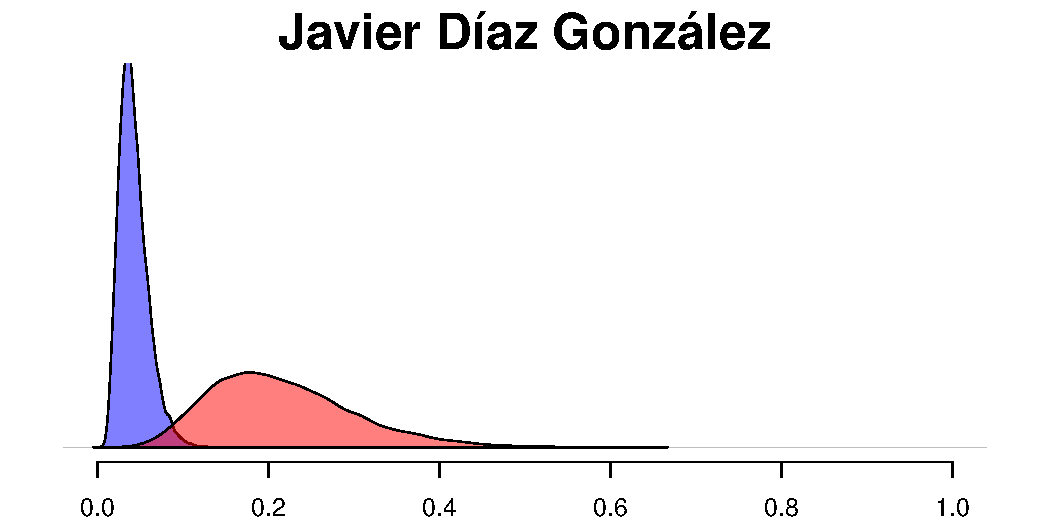
\includegraphics[width=.3\columnwidth]{../graphs/prReconoce1.pdf} &
    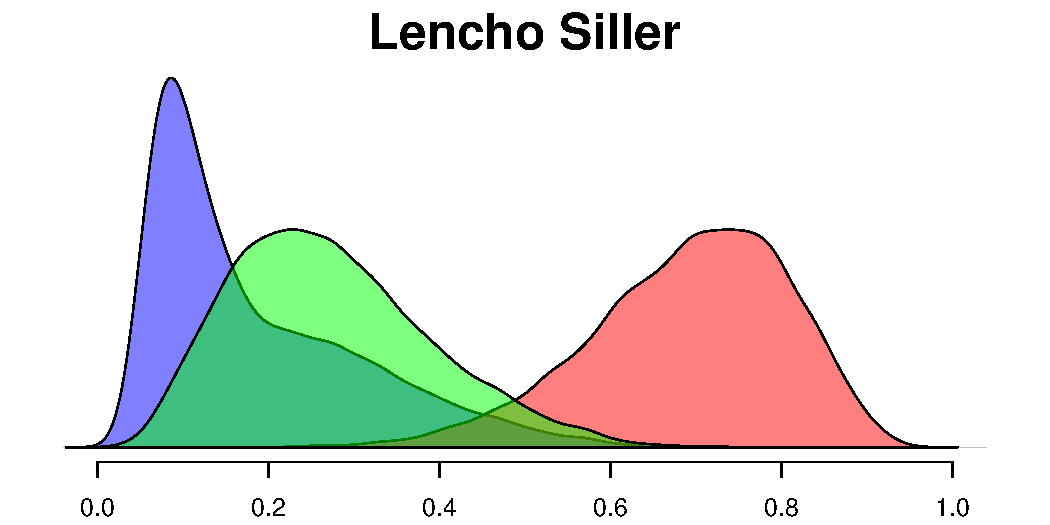
\includegraphics[width=.3\columnwidth]{../graphs/prReconoce6.pdf} &
    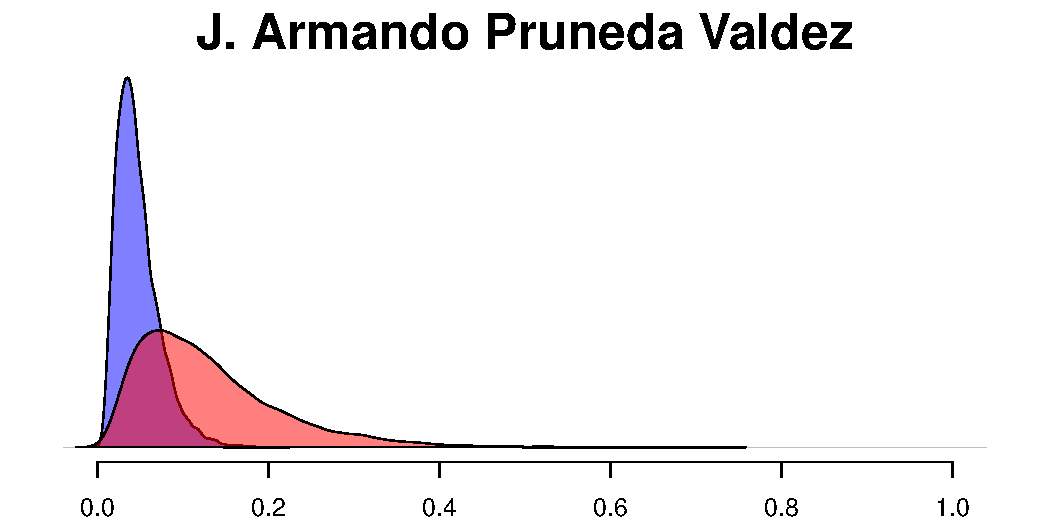
\includegraphics[width=.3\columnwidth]{../graphs/prReconoce8.pdf} \\
    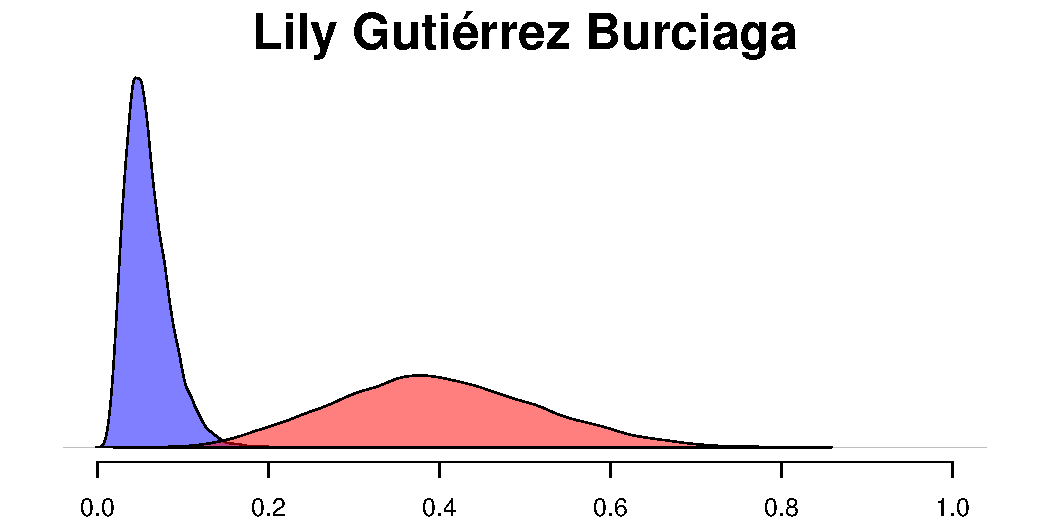
\includegraphics[width=.3\columnwidth]{../graphs/prReconoce2.pdf} &
    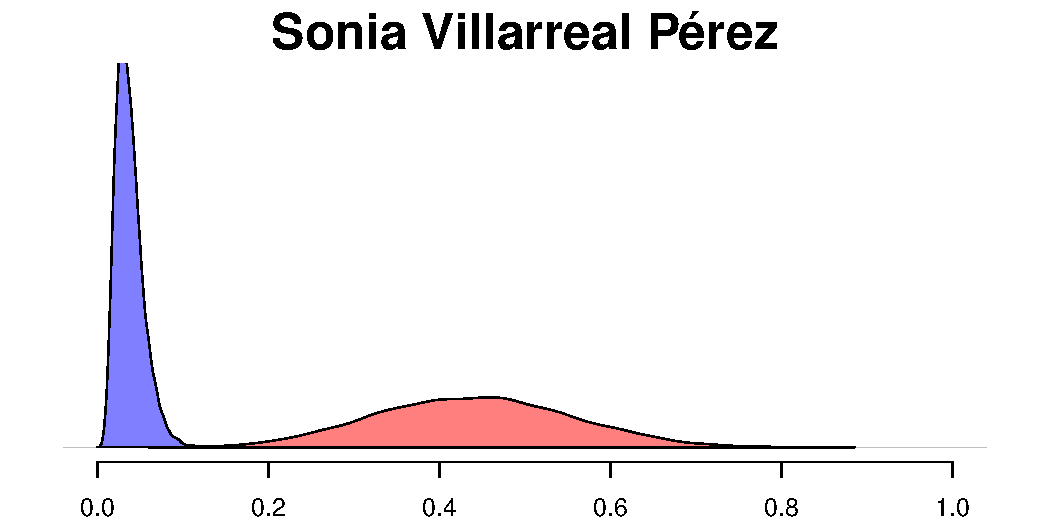
\includegraphics[width=.3\columnwidth]{../graphs/prReconoce5.pdf} &
    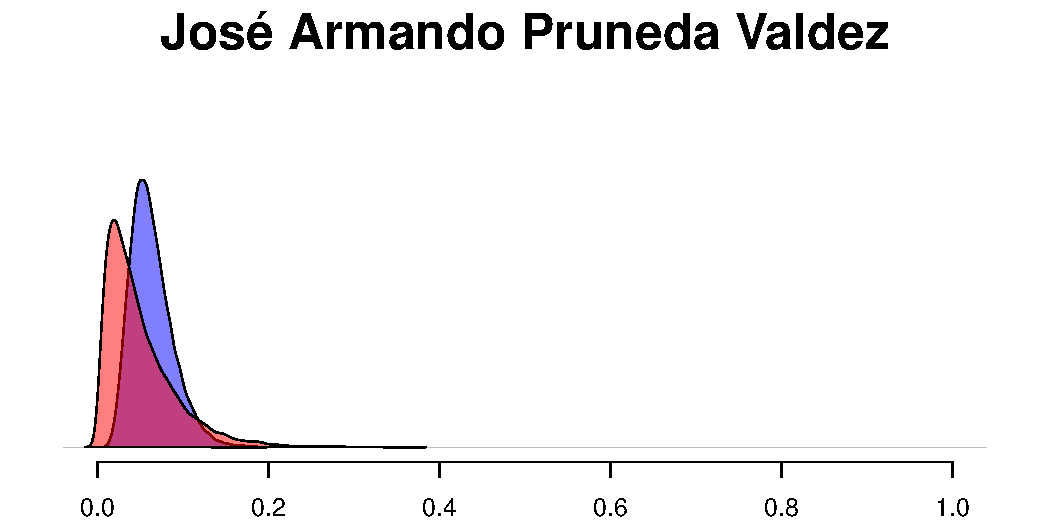
\includegraphics[width=.3\columnwidth]{../graphs/prReconoce7.pdf} \\
    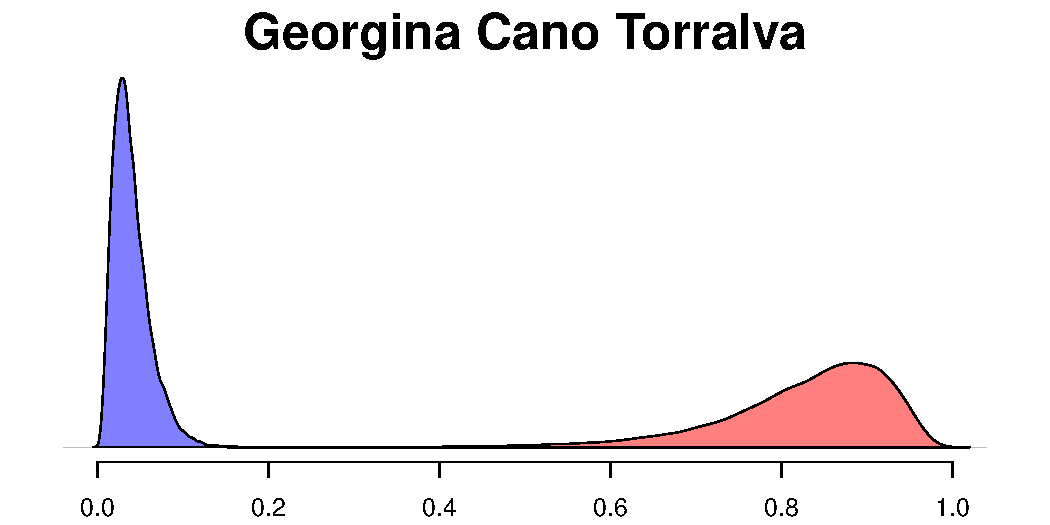
\includegraphics[width=.3\columnwidth]{../graphs/prReconoce3.pdf} &
    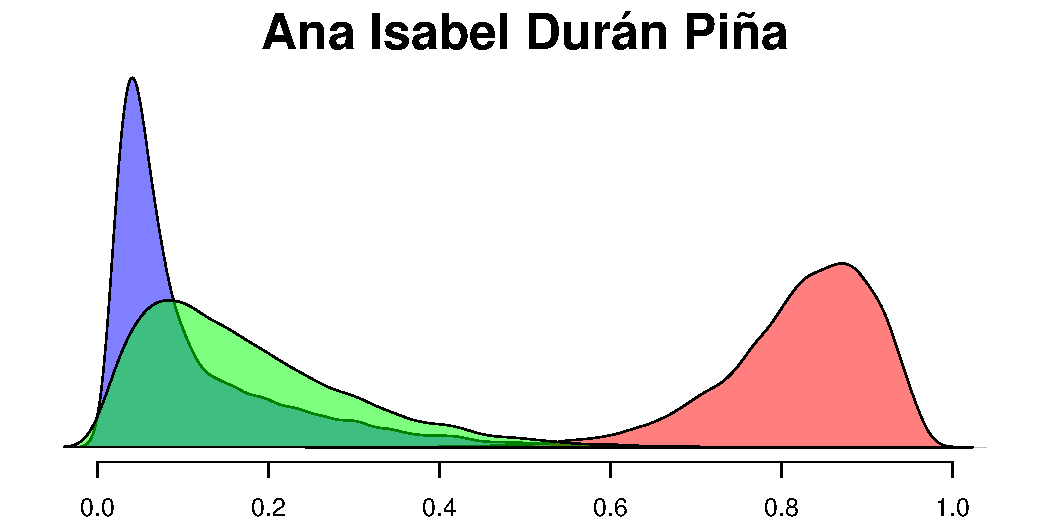
\includegraphics[width=.3\columnwidth]{../graphs/prReconoce4.pdf} &
    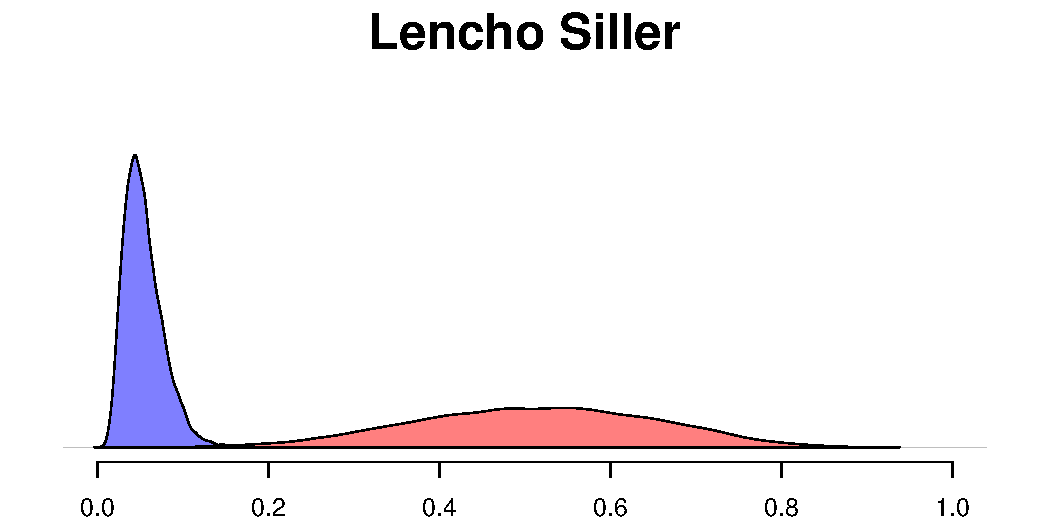
\includegraphics[width=.3\columnwidth]{../graphs/prReconoce9.pdf} \\
  \end{tabular}
  \caption{La probabilidad de reconocer al candidato. Representamos simulaciones a partir de la versión bayesiana de los modelos. La densidad violeta es para entrevistados en zona $h$, la mamey en zona $c$ y la verde (cuando aplica) en zona $p$. El eje horizontal mide la probabilidad de que el candidato sea reconocido por el entrevistado. Las demás variables del modelo fueron fijadas para representar un entrevistado que estima que el ocupante ha hecho algo por el distrito, sin interés en política, con smartphone, que simpatiza con el PAN.}\label{f:sims}
\end{sidewaysfigure}

Con reservas, los efectos son consistentes con la teoría. 

%% \begin{table}
%% \centering
%% \caption{One proposal and two amendments}\label{T:example}
%% \noindent \begin{tabular}{llc}
%%        & original version                   & amendment                                        \\ \hline
%% Art 1. & appropriate \$200                  & \$300                                            \\
%% Art 2. & split in two equal parts $(\frac{1}{2}, \frac{1}{2})$          & $(\frac{1}{4}, \frac{3}{4})$ split \\
%% Art 3. & one for students, one for teachers & ---                                              \\
%% \end{tabular}
%% \end{table}

%% \begin{figure}
%%   \centering
%%     \caption{The president rules game. The dashed branch may be practicable, or not.}\label{F:game}
%%     \tikzstyle{mid}=[circle,draw]
%%     \begin{tikzpicture}
%%       % \node[rectangle,draw] (n) at (0,0) {Nature};
%%       %\node (n) at (0,0) {\footnotesize{(Nature): $\pi$}};
%%       \node[mid] at (1.5,-0.25) (c) {\emph{C}};
%%       \node[mid] at (4,1) (p) {\emph{P}};
%%       \node[mid] at (6.5,1) (f) {\emph{F}};
%%       \node at (4,-1.5) (ce) {$q$};
%%       \node at (6.5,2.25) (pe1) {$x_F$};
%%       \node at (6.5,-0.25) (pe2) {$q$};
%%       \node at (9,2.25) (fe1) {$x_C$};
%%       \node at (9,-0.25) (fe2) {$q$};
%%       % \node at (0,0.7) {\small{Strategies:}}; \node at (2,0.7)
%%       % {\footnotesize{---}}; \node at (4,0.7) {\footnotesize{$x^*$}};
%%       % \node at (6,0.7) {\footnotesize{$y^*(x)$}}; \node at (8,0.7)
%%       % {\footnotesize{$z^*(x)$}}; \node at (0,-1.7)
%%       % {\small{Outcomes:}};
%%       %\path[->] (n) edge (c);
%%       \path[-] (c) edge node [above, sloped] {\footnotesize{report}} (p)
%%                (p) edge node [above, sloped] {\footnotesize{ur-}} (f)
%%                    edge node [below, sloped] {\footnotesize{gent}} (f);
%%       % \path[] (n) edge node [below] {\footnotesize{$\pi$}} (c)
%%       \path[] (c) edge node [below, sloped] {\footnotesize{$x_C$}} (p);
%%       \path[-o] (c) edge node [below, sloped] {\footnotesize{not}} (ce)
%%                 (p) edge node [above, sloped] {\footnotesize{standard}} (pe1)
%% %                    edge node [below, sloped] {\footnotesize{feto}} (pe2)
%%                 (f) edge node [above, sloped] {\footnotesize{accept}} (fe1)
%%                     %edge node [above, sloped] {\footnotesize{ofer-}} (fe2)
%%                     edge node [below, sloped] {\footnotesize{reject}} (fe2);
%%       \path[-o, dashed] (p) edge node [below, sloped] {\footnotesize{veto}} (pe2);
%%     \end{tikzpicture}
%% \end{figure}


% next command removes proportional font in table's superscripts
%(eval-after-load "tex-mode" '(fset 'tex-font-lock-suscript 'ignore)) 

% dv12 controlling for comm chair, executive bills only
% Table created by stargazer v.5.2 by Marek Hlavac, Harvard University. E-mail: hlavac at fas.harvard.edu
% Date and time: Wed, Aug 23, 2017 - 09:15:00 AM
% Requires LaTeX packages: dcolumn 
%% \begin{table}%[!htbp]
%%   \centering 
%%   \caption{Executive bill urgency predictors. Model 3 includes fixed Legislatura effects (not reported). Model 4 estimates separate error terms by Legislatura. Method of estimation: generalized linear model (model 4), others with logit.}\label{t:urgenLogit}
%%   \begin{tabular}{@{\extracolsep{0pt}}lD{.}{.}{-3} D{.}{.}{-3} D{.}{.}{-3} D{.}{.}{-3} } 
%%     \hline \\[-1.8ex] 
%%     & \multicolumn{4}{c}{DV: Bill received urgency (1) or not (0)} \\ 
%%     \\[-1.8ex] & \multicolumn{1}{c}{(1)} & \multicolumn{1}{c}{(2)} & \multicolumn{1}{c}{(3)} & \multicolumn{1}{c}{(4)}\\ 
%%     \\ [-1.8ex] 
%%     \hline \\[-1.8ex] 
%%     \emph{Co-partisan}     &  .333^{***} &  &  &                                        \\
%%     \emph{comm.~chair}     & (.009) &  &  &                                             \\ [.75ex]
%%     \emph{Coalition}       &  & 1.056^{***} & 1.139^{***} & 1.110^{***}                 \\
%%     \emph{comm.~chair}     &  & (<.001) & (<.001) & (<.001)                             \\ [.75ex]
%%     \emph{Multiple}        &  .603^{***} &  .623^{***} &  .631^{***} &  .631^{***}      \\
%%     \emph{referrals}       & (<.001) & (<.001) & (<.001) & (<.001)                      \\ [.75ex]
%%     \emph{Hacienda}        & 1.403^{***} & 1.324^{***} & 1.304^{***} & 1.308^{***}      \\
%%     \emph{referral}        & (<.001) & (<.001) & (<.001) & (<.001)                      \\ [.75ex]
%%     \emph{Pres.}           &  -.015 &  -.041 &  .029 &  .005                            \\
%%     \emph{approval}        & (.837) & (.567) & (.710) & (.945)                          \\ [.75ex]
%%     \emph{Introduced}      &  -.747^{***} &  -.733^{***} &  -.784^{***} &  -.771^{***}  \\
%%     \emph{in Senate}       & (<.001) & (<.001) & (<.001) & (<.001)                      \\ [.75ex]
%%     \emph{Senate}          &  -.303 &  -.382^{*} &  &                                   \\
%%     \emph{majority}        & (.136) & (.057) &  &                                       \\ [.75ex]
%%     \emph{Year}            &  .028 &  .020 &  .001 &  .002                              \\
%%     \emph{remaining}       & (.627) & (.737) & (.983) & (.974)                          \\ [.75ex]
%%     \emph{(Year}           &  -.242^{***} &  -.259^{***} &  -.275^{***} &  -.273^{***}  \\
%%     \emph{remaining)$^2$}  & (<.001) & (<.001) & (<.001) & (<.001)                      \\ [.75ex]
%%     \emph{Relax}           &  .647^{**} &  .591^{**} &  &                               \\
%%     \emph{deadlines}       & (.012) & (.018) &  &                                       \\ [.75ex]
%%     %% \emph{2002-06 Leg.} &  &  &  -.203 &                                             \\
%%     %%                     &  &  & (.298) &                                             \\ [.75ex]
%%     %% \emph{2006-10 Leg.} &  &  &  .302^{*} &                                          \\
%%     %%                     &  &  & (.097) &                                             \\ [.75ex]
%%     %% \emph{2010-14 Leg.} &  &  & 1.200^{***} &                                        \\
%%     %%                     &  &  & (<.001) &                                            \\ [.75ex]
%%     Intercept              &  -.743^{***} & -1.465^{***} & -1.977^{***} & -1.627^{***}  \\
%%                            & (.002) & (<.001) & (<.001) & (<.001)                       \\ [.75ex]
%%     \hline \\[-1.8ex] 
%%     Effects & \multicolumn{1}{c}{none} & \multicolumn{1}{c}{none} & \multicolumn{1}{c}{fixed} & \multicolumn{1}{c}{mixed} \\ 
%%     Observations & \multicolumn{1}{c}{1,461} & \multicolumn{1}{c}{1,461} & \multicolumn{1}{c}{1,461} & \multicolumn{1}{c}{1,461} \\ 
%%     Log$L$ & \multicolumn{1}{c}{-864} & \multicolumn{1}{c}{-860} & \multicolumn{1}{c}{-849} & \multicolumn{1}{c}{-857} \\ 
%%     \% correct & \multicolumn{1}{c}{90} & \multicolumn{1}{c}{90} & \multicolumn{1}{c}{90} & \multicolumn{1}{c}{90} \\ 
%% %%Akaike Inf. Crit. & \multicolumn{1}{c}{1,748.896} & \multicolumn{1}{c}{1,740.400} & \multicolumn{1}{c}{1,719.057} & \multicolumn{1}{c}{1,731.050} \\ 
%% %%Bayesian Inf. Crit. &  &  &  & \multicolumn{1}{c}{1,778.632} \\ 
%%     \\ [-1.8ex] 
%%     \hline \\[-1.8ex] 
%%     & \multicolumn{4}{r}{\footnotesize $^{*}$p$<$.1; $^{**}$p$<$.05; $^{***}$p$<$.01 (p-values in parentheses)} \\ 
%%   \end{tabular} 
%% \end{table} 


%% \begin{figure}
%%   \centering
%%     \caption{Average marginal effects from model 3. Dots report how the probability of an urgent bill changes in response to a unit change in each independent variable, all else at mean values; bars are 95-percent confidence intervals.}\label{F:avgMg}
%%     \includegraphics[width=.8\columnwidth]{../graphs/avgMgEffects.pdf}
%% \end{figure}

\bibliographystyle{apsrInitials}
\bibliography{/home/eric/Dropbox/mydocs/magar}

\end{document}
